% !TeX encoding = UTF-8
% !TeX root = V34_TEM.tex
% !TeX spellcheck = de_DE_frami

\section{Einleitung}
Die Transmissions-Elektronen-Mikroskopie (TEM) ermöglicht es, Bilder mit sehr großer Auflösung von atomaren Strukturen aufzunehmen. Man macht sich die Welleneigenschaft von stark beschleunigten Elektronen mittels der de-Broglie-Hypothese zunutze. Somit erreicht man Wellenlängen im Bereich von $\lambda=4\,\pico\metre$.
Die bisherigen Lichtmikroskope sind dagegen nur für das sichtbare Lichtspektrum von $\lambda=400\dots 700\,\nano\metre$ vorgesehen, was die Auflösung entsprechend begrenzt.\\
Analog zum Lichtmikroskop lassen sich in der Elektronenoptik ebenso Linsensysteme erstellen. Die Linsen werden dagegen von Magnetfeldern erzeugt, durch welche die Elektronen entsprechend abgelenkt werden. Im Gegensatz existieren nach einem Theorem von Scherzer nur konvexe Magnetolinsen, welche zudem bestimmte Aberrationen besitzen. Zudem muss für den optischen Weg der Elektronen ein Hochvakuum aufgebaut werden, welches die Untersuchung von lebenden biologischen Proben unmöglich macht. Es ist eine entsprechende Präparation der zu untersuchenden Proben notwendig.\\
Wir werden uns im folgenden Versuch im Wesentlichen mit der Funktionsweise des TEMs beschäftigen. Aufgrund einiger Analogien zwischen Lichtmikroskop und TEM werden wir zunächst ein klassisches optisches System aufbauen und die Prinzipien der geometrischen Optik sowie der Beugung von Licht, insbesondere die Fraunhofer Beugung, näher betrachten.
Im Anschluss studieren wir einige Betriebsmodi des TEM und nehmen entsprechend Bilder eines Siliziumgitters zur Kalibration und einer unbekannten metallischen Probe zur Bestimmung auf.
\section{Theorie}
\subsection{Geometrische Optik}
Auf makroskopischer Ebene in einem homogenen Medium lässt sich eine elektromagnetische Lichtwelle als Strahl ausgehend von der Quelle beschreiben. Diese breitet sich in Richtung des Wellenvektors aus. Für den Strahlengang durch eine dünne konvexe Linse gilt die Linsengleichung
\begin{align}
\frac{1}{f}=\frac{1}{g}+\frac{1}{b},
\label{eq:abb_gleichung}
\end{align}
wobei $f$ die Brennweite der Linse, $g$ die Gegenstandsweite zur Linse, und $b$ der entsprechende Abstand zur Linse ist. Für $g=\infty$, dies entspricht einen Strahl parallel zur optischen Achse, ist $b=f$. Ist dagegen $b=\infty$, so gilt $g=f$. Damit lassen sich optische Abbildungen wie in Abbildung \ref{fig:geo_optik} konstruieren.
\begin{figure}[h]
	\centering
	\includegraphics[width=0.8\textwidth]{linsengleichung.pdf}
	\caption{Konstruktion einer Abbildung mit der Linsengleichung.}
	\label{fig:geo_optik}
\end{figure}
Die Trajektorie eines Elektrons im TEM lässt sich in Näherung ebenso als geradlinigen Strahl beschreiben, weshalb die Betrachtung über die geometrische Optik zulässig ist.
\subsection{Abbildungsfehler}
Sowohl optische als auch magnetische Linsen sind im Allgemeinen nicht stigmatisch, d.h. ein Punkt der Gegenstandsebene wird nicht auf einem Punkt in der Bildebene abgebildet. Im folgenden lassen sich die Abbildungsfehler, die sogenannten \emph{Aberrationen}, grob in zwei Kategorien einteilen.
\subsubsection{Chromatische Aberration}
Dieser Fehler beruht auf der wellenlängenabhängigen Brechungszahl $n(\lambda)$ (\emph{Dispersion}). Die Linse besitzt für verschiedene Wellenlängen unterschiedliche Foki, dies ist in Abbildung \ref{fig:chromatic_abb} veranschaulicht.
Beheben lässt sich die chromatische Aberrationen bei optischen Linsen durch das Anbringen eines \emph{Achromaten}, eine konkave Linse mit einer anormalen Dispersion. Für magnetische Linsen existiert dagegen keine Korrektur dieser Art.
\subsubsection{Monochromatische Aberrationen}
Die Ursache dieser Aberrationen ist die Geometrie der durchlaufenden Linse.\\
\newline
\textbf{Sphärische Aberration}

Diese Aberration taucht bei den meisten sphärisch geschliffenen Linsen auf und hat als Ursache, dass achsenferne Strahlen nicht mehr der paraxialen Näherung genügen. Sie werden in einem anderen Brennpunkt fokussiert als achsennahe Strahlen (vgl. Abbildung \ref{fig:spheric_abb}), für welche die Abbildungsgleichung \eqref{eq:abb_gleichung} gilt.\\
Diese Aberration lässt sich minimieren durch
\begin{itemize}
	\item Unterdrückung der achsenfernen Strahlen mit z.B. einer Lochblende. Jedoch treten so Intensitätsverluste auf;
	\item Verwendung einer plankonvexen Linse, deren konvexen Seite der Gegenstandsseite zugewandt ist;
	\item eine Kombination von Sammel- und Zerstreuungslinsen;
	\item speziell geschliffene asphärische Linsen.
\end{itemize}


\textbf{Astigmatismus}

Der Abbildungsfehler entsteht, wenn das Objekt sich nicht auf der optischen Achse, sondern versetzt davon befindet. Dadurch fallen die Strahlenbündel schräg in die Linse, und es ergeben sich unterschiedliche Brennweiten in der sogenannten \emph{Meridional-} (M) und \emph{Sagittalebene} (S), wie in Abbildung \ref{fig:astigmatismus} veranschaulicht wird.\\

\textbf{Koma}

Betrachtet man nun auch die Strahlen, welche nicht achsenparallel in die Linse einfallen, so werden diese unterschiedlich an der Linse gebrochen und in einem anderem Bildpunkt der Bildebene fokussiert. Bei sphärischen Linsen entstehen dadurch Ringe, welche einen Schweif bilden (lat. \emph{coma}). Dies ist in Abbildung \ref{fig:koma} veranschaulicht. Die Koma ist eine Überlagerung der sphärischen Aberration und des Astigmatismus.
Sie kann gemildert werden durch Abdecken der achsenfernen Strahlen, jedoch bleibt so der Astigmatismus schiefer Bündel bestehen.

\begin{figure}[h]
	\centering
	\begin{subfigure}[b]{0.45\textwidth}
		\centering
		\includegraphics[width=\textwidth]{chromatic_abb.pdf}
		\caption{Chromatische Aberration.}
		\label{fig:chromatic_abb}
	\end{subfigure}
	\hfill
	\begin{subfigure}[b]{0.45\textwidth}
		\centering
		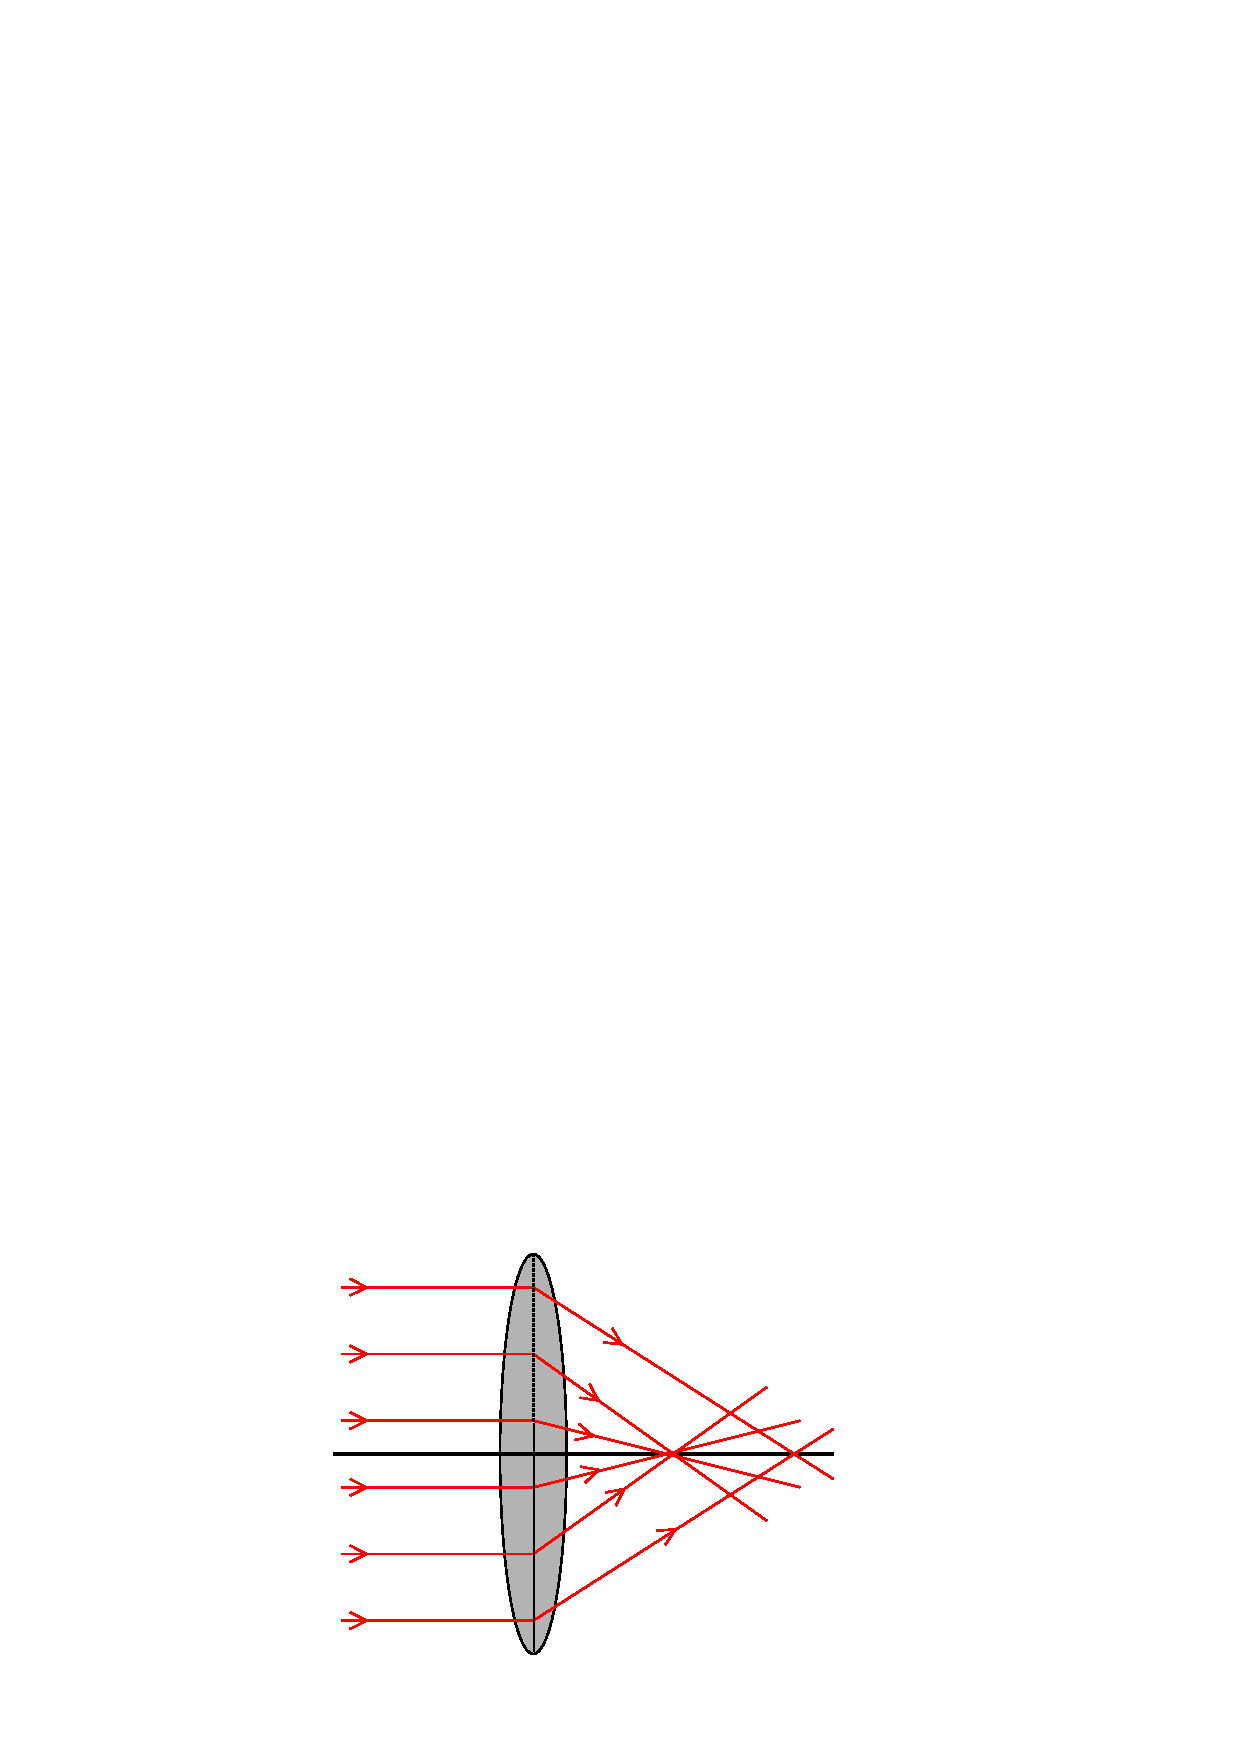
\includegraphics[width=\textwidth]{spheric_abb.pdf}
		\caption{Sphärische Aberration.}
		\label{fig:spheric_abb}
	\end{subfigure}
	
	\begin{subfigure}[b]{0.45\textwidth}
		\centering
		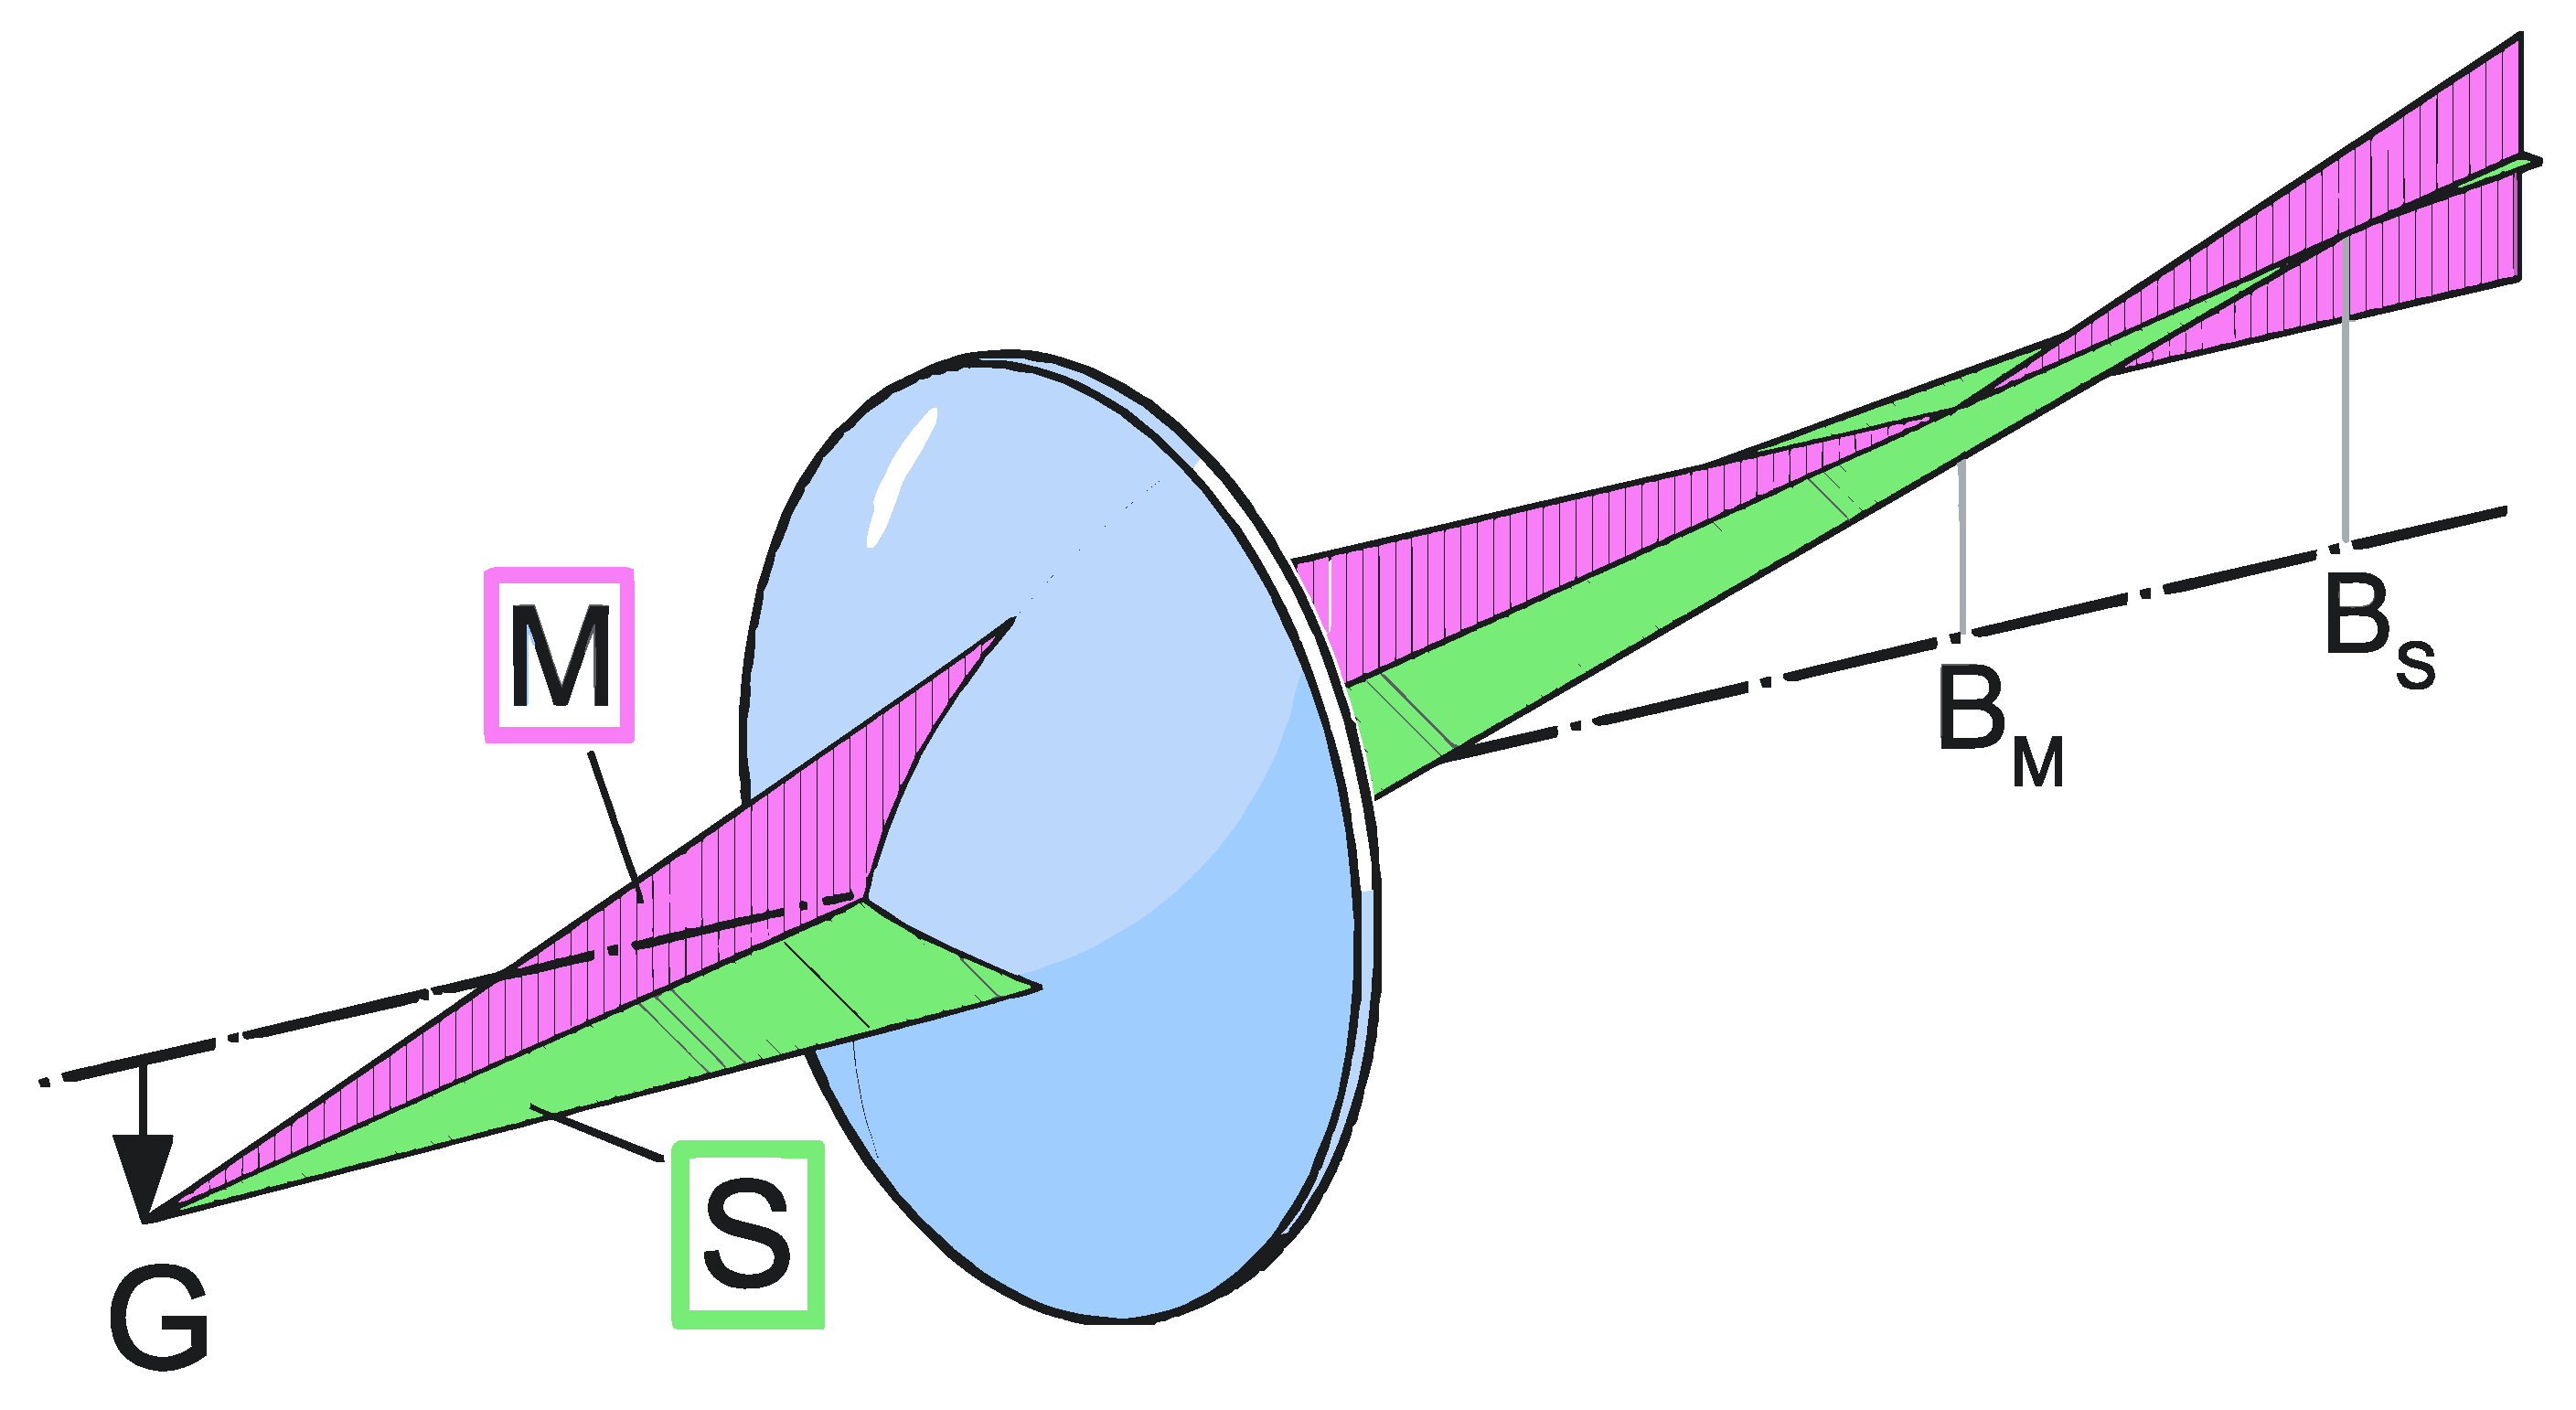
\includegraphics[width=\textwidth]{Meridional_SagittalPlane.pdf}
		\caption{Astigmatismus \cite{lit:wiki_astigma}.}
		\label{fig:astigmatismus}
	\end{subfigure}
	\hfill
	\begin{subfigure}[b]{0.45\textwidth}
		\centering
		\includegraphics[width=\textwidth]{koma.pdf}
		\caption{Koma.}
		\label{fig:koma}
	\end{subfigure}
	\caption{Abbildungsfehler in der geometrischen Optik.}
\end{figure}
\subsection{Beugung}
Wir betrachten im Folgenden die Beugung der elektromagnetischen Welle an einem Objekt. Aufgrund des Teilchen-Wellen-Dualismus gilt die Betrachtung auch für die im TEM beschleunigten Elektronen.
\subsubsection{Fraunhofer Beugung}
Wir gehen aus vom Sommerfeldschen Beugungsintegral
\begin{align}
U(P_0)=\frac{1}{\mathrm{i}\lambda}\iint\limits_\Sigma U(P_1)\frac{\exp(\mathrm{i}kr_{01})}{r_{01}}\cos\theta~\d \vec{s},
\end{align}
dabei sind $P_0$ und $P_1$ Ortspunkte der Bild- bzw. Beugungsebene, $U(P_0)$ die an dem Ort $P_0$ vorherrschende Feldstärke, $\vec{r}_{01}$ der Abstandsvektor zwischen $P_0$ und $P_1$ und $\theta$ der Winkel zwischen $\vec{r}_{01}$ und der optischen Achse. $\Sigma$ ist zudem die Fläche des beugenden Objekts und die Wellenzahl $k=\frac{2\pi}{\lambda}$. Eine ausführlichere Herleitung ist in \cite{lit:goodman96} zu finden.\\
Betrachten wir nun die Beugung im Fernfeld, d.h. der Abstand $d$ der Bild- zur Beugungsebene ist viel größer als die Abmessung des beugenden Objekts und des Beugungsbildes, so vereinfacht sich das Beugungsintegral zu
\begin{align}
U(x,y)=\underbrace{\frac{\exp(\mathrm{i}kd)\cdt\exp\left(\frac{\mathrm{i}k}{2d}(x^2+y^2)\right)}{\mathrm{i}kd}}_{A(x,y,d)}\iint\limits_{-\infty}^{\infty}U(\xi,\eta)\exp\left(-\mathrm{i}\frac{2\pi}{\lambda d}(x\xi +y\eta)\right)\d\xi\;\d\eta,
\end{align}
dies ist die Fraunhofer Näherung. Die sogenannte \emph{Blendenfunktion} $U(\xi,\eta)$ ist definiert durch
\begin{align}
U(\xi,\eta)=E(\xi,\eta)\cdt \tau(\xi,\eta),
\end{align}
$E(\xi,\eta)$ ist die Feldstärkenverteilung welche auf das beugende Objekt fällt, und $\tau(\xi,\eta)$ die \emph{Transmissionsfunktion}, welche über dessen Geometrie bestimmt ist. Nehmen wir an, dass die Feldstärkenverteilung homogen und normalisiert ist, und lassen $A(x,y,d)$ kurz außer Betracht, so stellt sich heraus, dass die Fraunhofer Beugung die Fouriertransformation des Objekts, an dem die Beugung stattfindet, ist.\\
Dies ist insofern wichtig, da eine Linsenabbildung ebenfalls Eigenschaften einer Fouriertransformation besitzt. Dies gilt folglich auch für das TEM.\\
Somit lassen sich die Beugungsbilder verschiedener Objekte berechnen. Dazu ist das folgende Theorem sehr nützlich.
\subsubsection{Faltungstheorem}
Für zwei Funktionen $f(x)$ und $g(x)$ ist die Faltung $(f*g)(x)$ definiert mit
\begin{align}
(f*g)(x)=\int\limits_{-\infty}^{\infty}f(t)g(x-t)~\d t.
\end{align}
Für die Fouriertransformierte $\mathcal{F}[~](\nu)$ der Faltung gilt dann
\begin{align}
\mathcal{F}[(f*g)(x)](\nu)=\mathcal{F}[f(x)](\nu)\cdt \mathcal{F}[g(x)](\nu).
\end{align}
Durch Einsetzen der inversen Fouriertransformierten lässt sich ebenso zeigen, dass gilt:
\begin{align}
\mathcal{F}[f(x)](\nu)* \mathcal{F}[g(x)](\nu)=\mathcal{F}[(f\cdt g)(x)](\nu).
\end{align}
Damit lassen sich u.a. Beugungsbilder von Objekten, die einer Modulierung unterliegen, wesentlich einfacher berechnen. Dies wird im folgenden Abschnitt gezeigt.
\subsubsection{Berechnung von Beugungsbildern}
Wir betrachten im Folgenden die Fouriertransformierten $\mathcal{F}[](\nu)$ verschiedener Geometrien, welche durch die Transmissionsfunktion $\tau(x)$ beschrieben werden.
$\nu$ bezeichnet im Folgenden die Ortsfrequenz.\\

\textbf{Beugung am einem Spalt}

Für den Spalt mit Breite $b$ ist die Transmissionsfunktion
\begin{align}
\tau(x)=\Theta\left(\frac{b}{2}-|x|\right),
\end{align}
wobei $\Theta(x)$ die Heaviside-Funktion ist. Die Fouriertransformierte ist
\begin{align}
\mathcal{F}[\tau(x)](\nu)&=\int\limits_{-\infty}^{\infty}\tau(x)\exp(-2\pi\mathrm{i}\nu x)\d x=\int\limits_{-\infty}^{\infty}\Theta\left(\frac{b}{2}-|x|\right)\exp(-2\pi\mathrm{i}\nu x)\d x\nonumber\\
&=\int\limits_{-\frac{b}{2}}^{\frac{b}{2}}\exp(-2\pi\mathrm{i}\nu x)\d x=
\dots=b \sinc(\pi b\nu)
\end{align}
mit der sinc-Funktion, welche definiert ist durch
\begin{align}
\sinc(x)=\frac{\sin(x)}{x}.
\end{align}

\textbf{Beugung an einem Gitter}

Ein unendlich großes ideales Gitter lässt sich durch die Transmissionsfunktion
\begin{align}
\tau(x)=\sum\limits_{n=-\infty}^\infty \delta(x-ng)
\end{align}
beschreiben, wobei $\delta(x)$ die Deltafunktion und $g$ die Gitterkonstante des Gitters ist. Diese Funktion nennt man den Delta- oder Dirac-Kamm. Dessen Fouriertransformation ist wiederum ein Dirac-Kamm, jedoch mit einer modifizierten Gitterkonstante.
Betrachten wir ein endliches Gitter mit einer endlichen Anzahl $N$ an infinitesimal dünnen Spalten. Dessen Transmissionsfunktion $\tau(x)$ lautet
\begin{align}
\tau(x)=\sum\limits_{n=0}^{N-1} \delta(x-ng).
\end{align}
Die Fouriertransformierte ist entsprechend
\begin{align}
\mathcal{F}[\tau(x)](\nu)&=\int\limits_{-\infty}^{\infty}\sum\limits_{n=0}^{N-1} \delta(x-ng)\exp(-2\pi\mathrm{i}\nu x)\d x=\sum\limits_{n=-0}^{N-1}\exp(-\mathrm{i}2\pi\nu ng)\nonumber\\
&=\frac{\exp(\mathrm{i}2\pi\nu gN)-1}{\exp(\mathrm{i}2\pi\nu g)-1}=\dots =\exp(-\mathrm{i}\pi\nu g(N-1))\cdt \frac{\sin(\pi\nu gN)}{\sin(\pi\nu g)}.
\end{align}
In der Praxis haben die Gitterspalte eine endliche Breite $b$, vergleichbar mit einem Einzelspalt. Hier können wir das Faltungstheorem anwenden, und das Fraunhofer Beugungsbild des endlichen realen Gitters ist entsprechend
\begin{align}
\mathcal{F}[\tau(x)](\nu)=b~\exp(-\mathrm{i}\pi\nu g(N-1))\cdt \frac{\sin(\pi\nu gN)}{\sin(\pi\nu g)} \sinc(\pi b\nu).
\end{align}

\textbf{Beugung an zweidimensionalen Objekten}

Die Fraunhofer Beugung an zweidimensionalen Objekten lässt sich analog zum eindimensionalen berechnen. Hierzu wenden wir die zweidimensionale Fouriertransformation auf die Transmissionsfunktion $\tau(q_1,q_2)$ an, wobei $q_1,~q_2$ entsprechend gewählte allgemeine Koordinaten sind. Dadurch lässt sich der Integrand separieren.\\
Beispielsweise lässt sich ein rechteckiges Objekt als senkrechte Überlagerung von zwei Spalten auffassen. Oft wird eine Koordinatentransformation in Polarkoordinaten durchgeführt, beispielsweise für den Fall der Beugung an einer Lochblende mit Radius $\rho_0$. Dessen Transmissionsfunktion $\tau(\rho)$ ist definiert durch
\begin{align}
\tau(\rho)=\mathrm{circ}\left(\frac{\rho}{\rho_0}\right)
\end{align}
mit der Kreisfunktion
\begin{align}
\mathrm{circ}(x)=\left\{
	\begin{array}{l l}
	1 \quad x\le 1\\
	0 \quad x > 1
	\end{array}
	\right. .
\end{align}
Die Fouriertransformierte der Lochblende ist dann
\begin{align}
\mathcal{F}[\tau(\rho)](r,d)=\dots =2\pi\rho_0^2\cdt\frac{J_1\left(\frac{kr\rho_0}{d}\right)}{\frac{kr\rho_0}{d}},
\end{align}
hierbei ist $J_1(x)$ die \emph{Bessel-}Funktion erster Ordnung und erster Art, $d$ wiederum der Abstand der Lochblende zur Bildebene und $r$ die radiale Koordinate in der Bildebene.
\subsubsection{Bragg-Beugung}
Wir betrachten nun die Beugung einer Welle an einem (nicht absorbierenden) dreidimensionalen Objekt. Für den Versuch wird die Beugung in einem Kristallgitter behandelt. Dieses bildet mit den das Gitter bildenden Kristallatomen sogenannte $\emph{Netzebenen}$ aus. Diese hängen von der Kristallstruktur bzw. deren Einheitszellen ab.\\
Zur Charakterisierung der Kristallstruktur verwendet man die Basisvektoren $\vec{a}_1,~\vec{a}_2$ und $\vec{a}_3$, welche die Einheitszelle bilden. Im reziproken Raum definiert man sich entsprechend die reziproken Basisvektoren $\vec{g}_1,~\vec{g}_2,~\vec{g}_3$ mit
\begin{align}
\vec{g}_1=2\pi\frac{\vec{a}_2\times\vec{a}_3}{\left|\vec{a}_1\cdt (\vec{a}_2\times\vec{a}_3)\right|}\quad
\vec{g}_2=2\pi\frac{\vec{a}_3\times\vec{a}_1}{\left|\vec{a}_1\cdt (\vec{a}_2\times\vec{a}_3)\right|}\quad
\vec{g}_3=2\pi\frac{\vec{a}_1\times\vec{a}_2}{\left|\vec{a}_1\cdt (\vec{a}_2\times\vec{a}_3)\right|}.
\end{align}
Die Netzebenen werden durch den reziproken Gittervektor $\vec{G}$ beschrieben mit
\begin{align}
\vec{G}=h\vec{g}_1+k\vec{g}_2+l\vec{g}_3,
\end{align}
dabei sind $h,~k,~l$ die \emph{Miller-Indizes}. Der Gittervektor steht senkrecht zur Netzebene.\\
Der \emph{Netzebenenabstand} ist im Allgemeinen gegeben durch
\begin{align}
d_{hkl}=\frac{1}{\sqrt{\left(\frac{h}{a}\right)^2+\left(\frac{k}{b}\right)^2+\left(\frac{l}{c}\right)^2}},
\end{align}
wobei $a,~b,~c$ die Beträge der Basisvektoren in einem orthogonalen Koordinatensystem sind. Für ein kubisches Gitter (u.a. bei Kristallen mit fcc und bcc-Struktur) mit $a=b=c$ vereinfacht sich der Ausdruck zu
\begin{align}
d_{hkl}=\frac{a}{\sqrt{h^2+k^2+l^2}}.
\end{align}
$a$ ist somit auch die Gitterkonstante.\\
Die \emph{Bragg-Bedingung} beschreibt den Zusammenhang zwischen den Netzebenenabstand und dem Beugungswinkel. Sie ist gegeben durch
\begin{align}
n\lambda=2d_{hkl}\cos\theta,
\end{align}
dabei ist $n$ die Beugungsordnung und $\theta$ der Winkel zur Netzebene.
Äquivalent lässt sich im reziproken Raum die \emph{Laue-Bedingung} formulieren:
\begin{align}
\vec{k}-\vec{k_0}=\vec{G}
\end{align}
Wichtig ist zu beachten, dass im Gegensatz zur Röntgenbeugung die Elektronenbeugung aufgrund der viel kleineren de-Broglie-Wellenlänge relativ schwach ist (vgl. \autoref{fig:laue_bedingung}).
\begin{figure}[h]
	\centering
	\includegraphics[width=0.8\textwidth]{laue_bedingung.pdf}
	\caption[Laue-Bedingung]{Veranschaulichung der Laue-Bedingung im reziproken Raum mit der Ewald-Kugel.}
	\label{fig:laue_bedingung}
\end{figure}
\subsection{Kikuchi-Linien}
Die Kikuchi-Linien entstehen im TEM durch Mehrfachstreuung von Elektronen, vor allem bei dickeren Proben. Hier wird ein Teil der Elektronen elastisch gestreut nach der Laue-Bedingung, wodurch sich im Beugungsbild weitgehend diskrete Beugungsreflexe ergeben. Diese sind durch paarweise parallel verlaufende Kikuchi-Linien, welche Bänder bilden, verbunden. Sie entstehen durch inelastische Streuung der Elektronen, dabei streuen sie diffus in alle Richtungen und werden anschließend an den Netzebenen wieder elastisch gestreut (Bragg-Beugung).
Aufgrund dessen kann jeder Kikuchi-Linie die Miller-Indizes der Netzebenenschar, an dem die Beugung stattfand, zugeordnet werden. Die Breite der Bänder hängt zudem im Wesentlichen vom Verhältnis der Wellenlänge $\lambda$ zum Netzebenenabstand $d_{hkl}$ ab.